\documentclass{article}

% Course report: "preprint" shows author names and removes line numbers.
% For an anonymized NeurIPS-style submission, use \usepackage{neurips_2026} instead.
\usepackage[preprint]{neurips_2026}

\usepackage[utf8]{inputenc} % allow utf-8 input
\usepackage[T1]{fontenc}    % use 8-bit T1 fonts
\usepackage{hyperref}       % hyperlinks
\usepackage{url}            % simple URL typesetting
\usepackage{booktabs}       % professional-quality tables
\usepackage{amsfonts}       % blackboard math symbols
\usepackage{amsmath}
\usepackage{nicefrac}       % compact symbols for 1/2, etc.
\usepackage{microtype}      % microtypography
\usepackage{xcolor}         % colors
\usepackage{graphicx}

\title{Learning Where to Adapt: Attribute-Guided Test-Time Adaptation for 3D Foundation Models}

% TODO: replace with the actual author name(s), affiliation and email(s).
\author{%
  Author Name(s) \\
  DA4022 Final Project Report \\
  \texttt{email@institution.edu} \\
}

\begin{document}

\maketitle

\begin{abstract}
We investigate whether reusable adaptation directions can improve sparse-depth completion with a pretrained 3D foundation model (VGGT). We combine sparse-depth-guided test-time adaptation with fixed subspaces extracted from adapters trained under controlled geometry, camera, texture, and lighting variations. The study includes a known-optimum optimization experiment, synthetic attribute generation, transfer to real ScanNet images, a residual-LoRA extension, and sparsity and outlier evaluations. The strongest fixed-subspace method reaches \textbf{0.8967\%} unobserved-region absolute relative error, compared with \textbf{0.9739\%} for ordinary rank-4 LoRA, while optimizing only \textbf{384} instead of \textbf{393,216} parameters: \textbf{7.92\% lower error with 1,024$\times$ fewer trainable parameters}. The results also identify limits: benefits depend on the observation regime, combining attributes does not automatically help, and parameter savings do not translate into a substantial runtime reduction.
\end{abstract}

\section{Introduction}

Sparse-depth completion turns a limited set of depth measurements into a dense prediction. A pretrained 3D foundation model provides a strong geometric prior, but its predictions may still need scene-specific correction. Ordinary LoRA expresses that correction through low-rank factors learned afresh for every input. We ask whether useful correction directions can instead be learned beforehand and reused. The project connects two ideas: \textbf{CAPA}~[1], where sparse observations supervise test-time adaptation of a frozen model, and \textbf{attribute-subspace mining}~[2], where controlled 3D variations yield reusable directions for parameter-efficient adaptation. Our central question is:

\begin{quote}
\emph{Can attribute-derived fixed subspaces guide adaptation on held-out scenes while preserving prediction quality and reducing the number of parameters optimized at test time?}
\end{quote}

We examine both the benefits of restricting adaptation and the cost of an incomplete or mismatched subspace, and add a small residual LoRA to test whether scene-specific flexibility can compensate. Our contributions are:
\begin{itemize}
\item a fixed-subspace test-time adaptation scheme for VGGT that optimizes only 384 coefficients, with bases mined from controlled synthetic attribute variations;
\item a known-optimum quadratic study showing when a constrained search space preserves the optimum;
\item a held-out ScanNet evaluation against LoRA, random-basis, real-donor, and residual-hybrid controls, including sparsity, outlier, attribute, and efficiency analyses.
\end{itemize}

\section{Method}

\paragraph{Fixed-subspace adaptation.} For a frozen projection $W$, ordinary LoRA learns $W' = W + 2BA$ with trainable low-rank $A, B$ (the factor of two is the adapter scaling). Our formulation instead uses
\begin{equation}
W' = W + 2\,U M V^\top,
\end{equation}
where $U$ and $V$ are precomputed orthonormal bases and only $M$ is optimized for the target image. We adapt the QKV projections in 24 layers of VGGT's image encoder~[3]. With four-dimensional bases, each layer needs a $4\times4$ matrix, giving $24\times4\times4=384$ trainable coefficients versus 393,216 for rank-4 LoRA.

\paragraph{Controlled attribute data and basis extraction.} A procedural renderer generates scenes with room surfaces, a box, and a sphere, provides exact depth, and supports controlled interventions in four attribute families: \emph{geometry} (object size and placement), \emph{camera} (position and viewpoint), \emph{texture} (surface-pattern frequency), and \emph{lighting} (illumination direction). We use two base scenes and three intervention levels per attribute; other parameters stay fixed and one donor adapter is optimized across the three variants. No test-scene depth is used to extract bases. We compare two extraction strategies. (1) \emph{Robust shared-update bases}: a rank-constrained shared update is estimated with five iteratively reweighted least-squares iterations, and its singular directions define the bases. (2) \emph{Energy-pooled bases}: donor updates are Frobenius-normalized and their leading left and right update-energy directions are pooled separately, retaining variation across donors rather than a central correction. Individual and combined attribute bases use the same four-dimensional representation. Shared bases learned from real donor scenes provide an additional comparison.

\paragraph{Residual-LoRA hybrid.} A fixed basis may omit a correction a new scene needs. We therefore also test $W' = W + 2UMV^\top + 2B_{\mathrm{res}}A_{\mathrm{res}}$ with a rank-1 residual (98,688 parameters), against ordinary rank-1 LoRA (98,304) as a nearly matched control.

\paragraph{Sparse supervision and metric.} At test time, scale and shift are estimated from the sparse measurements, and adaptation minimizes depth error at those locations only. Measurements are simulated by sampling valid ground-truth pixels; corruption is applied only to the observed subset. The primary metric is absolute relative error on valid pixels \emph{outside} the conditioning set, so we evaluate the completion itself (lower is better):
\begin{equation}
\operatorname{AbsRel}(\%)=\frac{100}{|\Omega_{\mathrm{unobs}}|}\sum_{i\in\Omega_{\mathrm{unobs}}}\frac{|\widehat D_i-D_i|}{D_i}.
\end{equation}

\section{Experimental setup}

ScanNet sequences are split into disjoint roles (Table~\ref{tab:split}); no sequence crosses groups.

\begin{table}[h]
  \caption{Separation of learning, selection, and testing data.}
  \label{tab:split}
  \centering
  \small
  \begin{tabular}{lll}
    \toprule
    Role & ScanNet sequences & Purpose \\
    \midrule
    Real donors & \texttt{scene0707}, \texttt{scene0766} & Learn reusable real-scene update directions \\
    Validation & \texttt{scene0771} & Select learning rates; diagnose attribute bases \\
    Test & \texttt{scene0777}, \texttt{scene0806} & Evaluate selected methods on held-out sequences \\
    \bottomrule
  \end{tabular}
\end{table}
 ``Held-out'' refers to the project's own splits, not VGGT's pretraining data. Learning rates are selected on validation at a common 30-update budget and frozen; test scores are taken at the fixed final budget, never the best test checkpoint.

The \textbf{main comparison} uses two frames from each test sequence, two seeds for adapted methods, 100 updates, and 100 clean points. All 60 planned runs (56 adaptation runs over seven methods plus four frozen predictions) completed with no failures. Frame results are averaged within each sequence before averaging across sequences. The \textbf{sparsity} study uses the first selected frame per test sequence, one seed, 30 updates, and 20/100/500 points. The \textbf{outlier} study uses the same subset with 100 points and 0/10/20\% corruption, where observed values are multiplied by factors drawn uniformly from $[0.2, 2.0]$; locations and corruption are shared across methods. The \textbf{attribute ablation} uses two validation frames, 30 updates, and equal basis dimensions.

\section{Controlled optimization: when does a constraint preserve the optimum?}

Before the nonlinear model, we study a positive-definite quadratic with a known optimum: 60 ambient parameters, a six-dimensional constrained space, ten seeds, at most 1,500 gradient steps, a shared curvature-based learning-rate rule, and a target normalized gap of $10^{-6}$ (Table~\ref{tab:quad}).

\begin{table}[h]
  \caption{Quadratic with known optimum. Only the aligned subspace reaches the target; good conditioning alone is not enough.}
  \label{tab:quad}
  \centering
  \small
  \begin{tabular}{lccc}
    \toprule
    Search space & Runs reaching target & Median updates & Median eff.\ condition no. \\
    \midrule
    Full space & 0/10 (budget) & -- & 10,000.00 \\
    \textbf{Aligned (contains optimum)} & \textbf{10/10} & \textbf{25} & \textbf{8.71} \\
    Misaligned & 0/10 & -- & 9.64 \\
    Random & 0/10 & -- & 5.10 \\
    \bottomrule
  \end{tabular}
\end{table}

The aligned subspace preserves the optimum while improving conditioning. Misaligned and random subspaces are well conditioned but converge to inferior constrained solutions, with median best normalized gaps of about 0.205 and 0.687. The full-space optimum remains attainable but was not reached within budget. \textbf{Conditioning and representational capacity must be considered together}: a small search space helps only if it retains the needed correction. This experiment illustrates the mechanism; it is not a global-optimum guarantee for VGGT.

\section{Results}

\paragraph{Main result.} Table~\ref{tab:main} shows that reusable fixed bases support effective adaptation outside the observed pixels. Energy-pooled bases achieve the lowest mean error: a \textbf{7.92\% relative reduction} over rank-4 LoRA (0.0772 percentage points) with \textbf{99.90\% fewer} trainable parameters, and a 53.04\% reduction over the frozen model. At the same 384-parameter budget, they are \textbf{9.33\% better than random bases}, so the choice of directions matters beyond reducing capacity. Energy pooling also beats robust shared-update extraction (0.8967\% vs.\ 0.9398\%); a plausible reason is that preserving several donor variations is more useful than a single central correction, though the experiment does not isolate this cause. The hybrid improves 1.65\% over the nearly parameter-matched rank-1 LoRA, but only 0.00125 points over pure robust bases despite far more parameters. Figure~\ref{fig:qual} shows a qualitative example.

\begin{table}[h]
  \caption{Main comparison on held-out ScanNet test sequences (100 updates, 100 clean points). Energy-pooled fixed bases give the best mean error with 1,024$\times$ fewer trainable parameters than rank-4 LoRA.}
  \label{tab:main}
  \centering
  \small
  \begin{tabular}{lrrr}
    \toprule
    Method & Unobs.\ AbsRel (\%) $\downarrow$ & Trainable params & vs.\ rank-4 LoRA \\
    \midrule
    Aligned frozen VGGT & 1.9093 & 0 & -- \\
    Ordinary rank-4 LoRA & 0.9739 & 393,216 & reference \\
    Ordinary rank-1 LoRA & 0.9542 & 98,304 & 4$\times$ fewer \\
    Random fixed bases & 0.9890 & 384 & 1,024$\times$ fewer \\
    Real-donor shared bases & 0.9506 & 384 & 1,024$\times$ fewer \\
    Synthetic robust shared-update bases & 0.9398 & 384 & 1,024$\times$ fewer \\
    Synthetic bases + residual LoRA & 0.9385 & 98,688 & $\approx$3.98$\times$ fewer \\
    \textbf{Synthetic energy-pooled bases} & \textbf{0.8967} & \textbf{384} & \textbf{1,024$\times$ fewer} \\
    \bottomrule
  \end{tabular}
\end{table}

\begin{figure}[h]
  \centering
  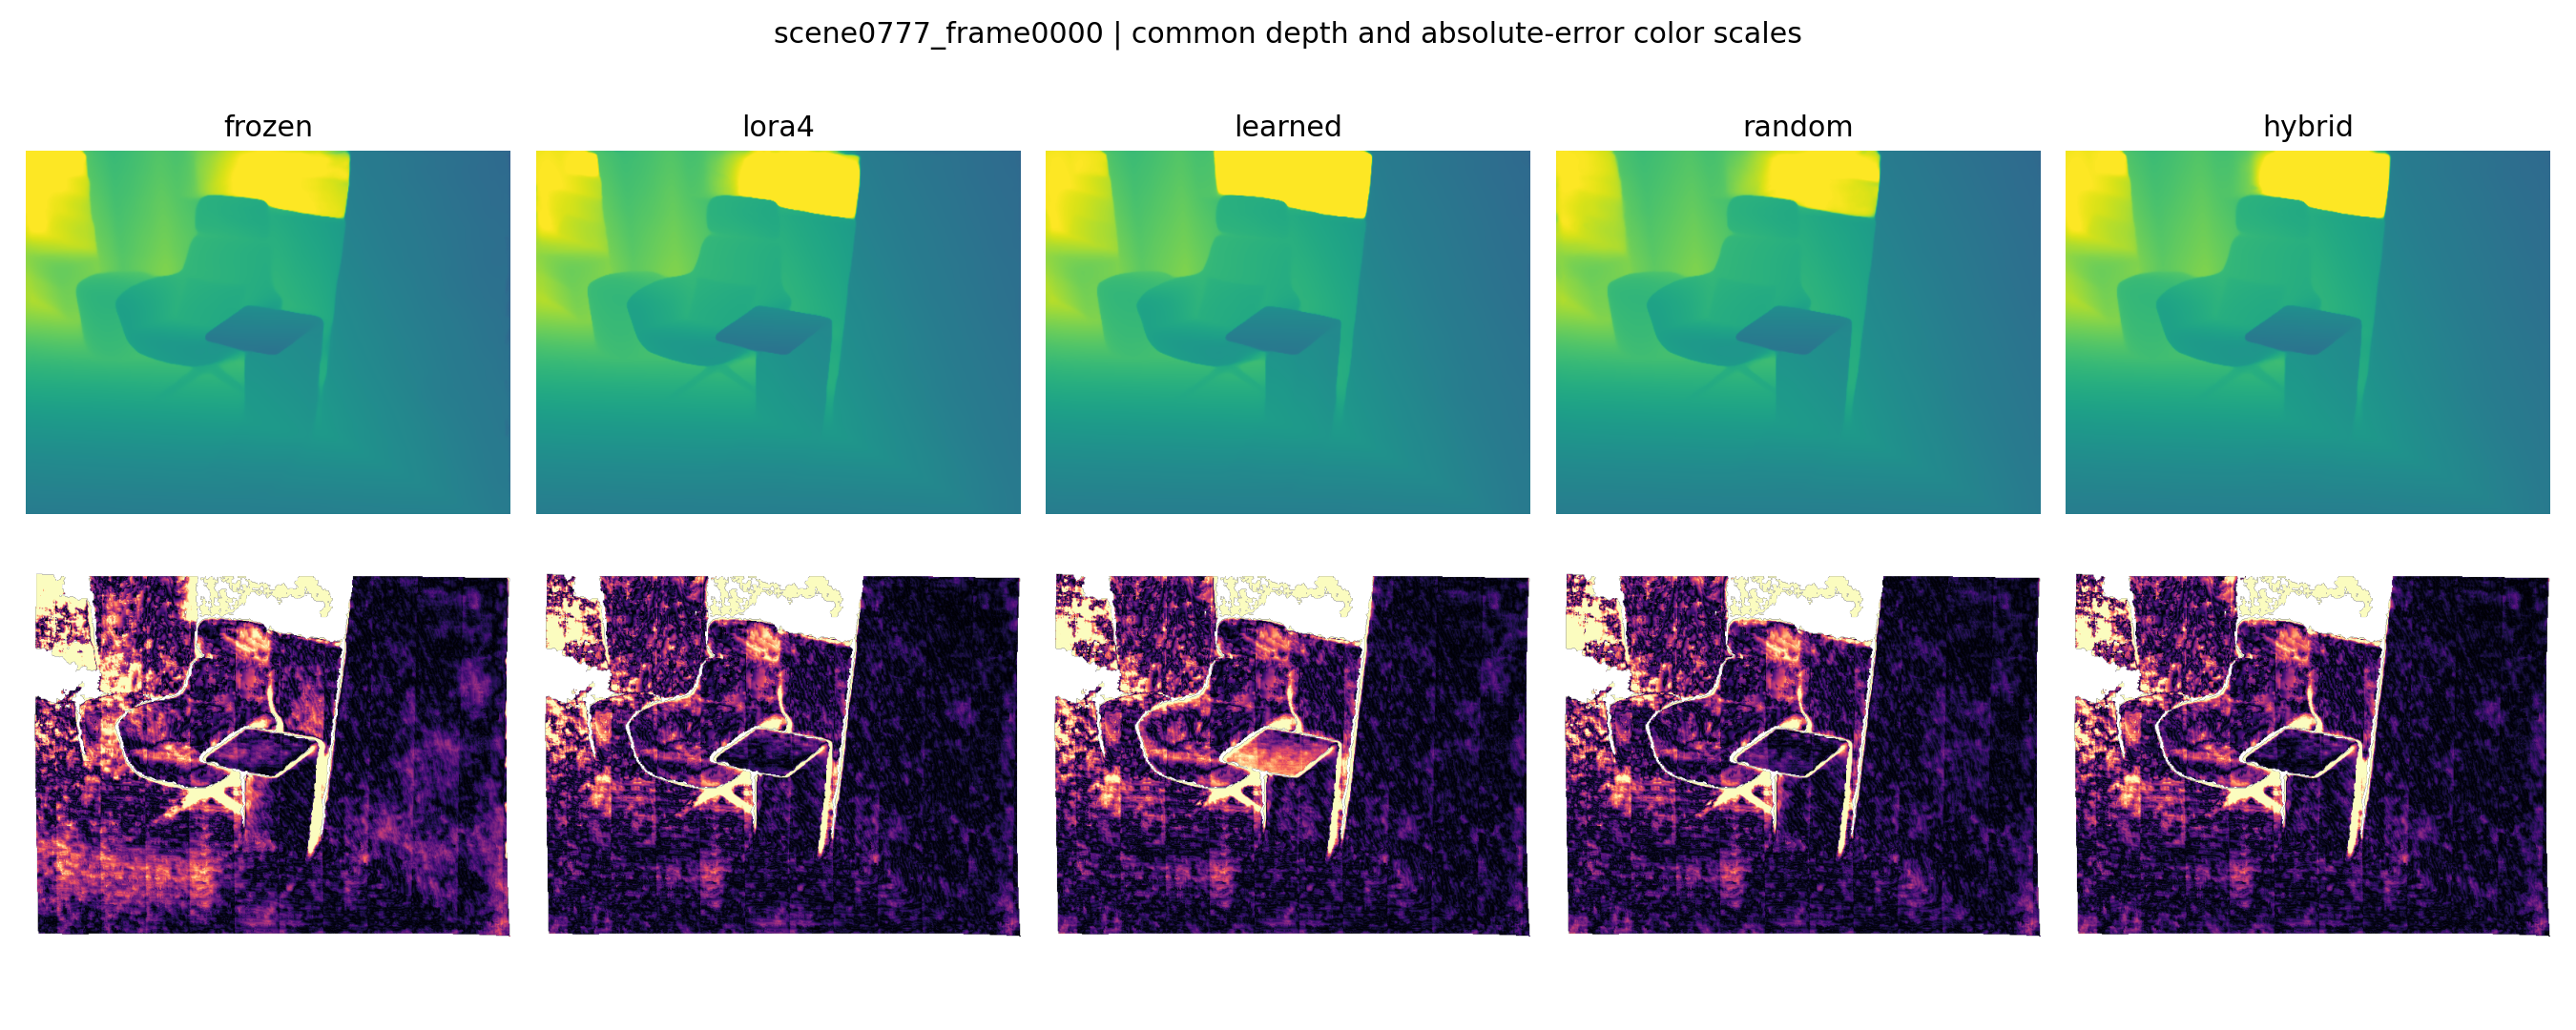
\includegraphics[width=0.92\linewidth, trim=0 30 0 40, clip]{qualitative.png}
  \caption{Test frame \texttt{scene0777} frame 0 with common color scales. Top: predicted depth. Bottom: absolute error (brighter is worse) for the frozen model, rank-4 LoRA, learned fixed bases, random bases, and the hybrid. Adaptation removes most of the frozen model's low-frequency error.}
  \label{fig:qual}
\end{figure}

\paragraph{Sparsity and outliers.} Table~\ref{tab:robust} and Figure~\ref{fig:robust} use a separate 30-update budget, so its values are not comparable to Table~\ref{tab:main}. The preferred adaptation space depends on the available evidence. At \textbf{100 points}, learned fixed bases give the lowest error. At \textbf{20 points}, random bases are best; adding the residual improves pure learned bases by 12.33\%, but random bases remain slightly better. At \textbf{500 points}, ordinary LoRA wins, since a more flexible space can exploit the extra evidence. Under corruption, learned bases stay almost unchanged between clean and 20\% outliers (1.0842\% vs.\ 1.0871\%) and are 6.66\% better than LoRA at 20\%. Some corrupted settings score better than clean ones; with two scenes and one corruption seed, we treat this as noise in a small experiment.

\begin{table}[h]
  \caption{Unobserved AbsRel (\%) by number of sparse points (clean) and outlier rate (100 points); 30 updates. No single adaptation space wins every regime.}
  \label{tab:robust}
  \centering
  \small
  \begin{tabular}{lccccc}
    \toprule
    & \multicolumn{3}{c}{Sparse points} & \multicolumn{2}{c}{Outlier rate} \\
    \cmidrule(lr){2-4} \cmidrule(lr){5-6}
    Method & 20 & 100 & 500 & 10\% & 20\% \\
    \midrule
    Aligned frozen VGGT & 1.4903 & 1.4823 & 1.4726 & 1.4959 & 1.5027 \\
    Ordinary rank-4 LoRA & 1.3077 & 1.1458 & \textbf{0.7285} & 1.1184 & 1.1646 \\
    Synthetic robust bases & 1.3584 & \textbf{1.0842} & 0.8348 & 1.0691 & \textbf{1.0871} \\
    Random fixed bases & \textbf{1.1784} & 1.1442 & 0.7996 & 1.1513 & 1.1842 \\
    Synthetic bases + residual & 1.1908 & 1.0928 & 0.7657 & \textbf{1.0623} & 1.1164 \\
    \bottomrule
  \end{tabular}
\end{table}

\begin{figure}[h]
  \centering
  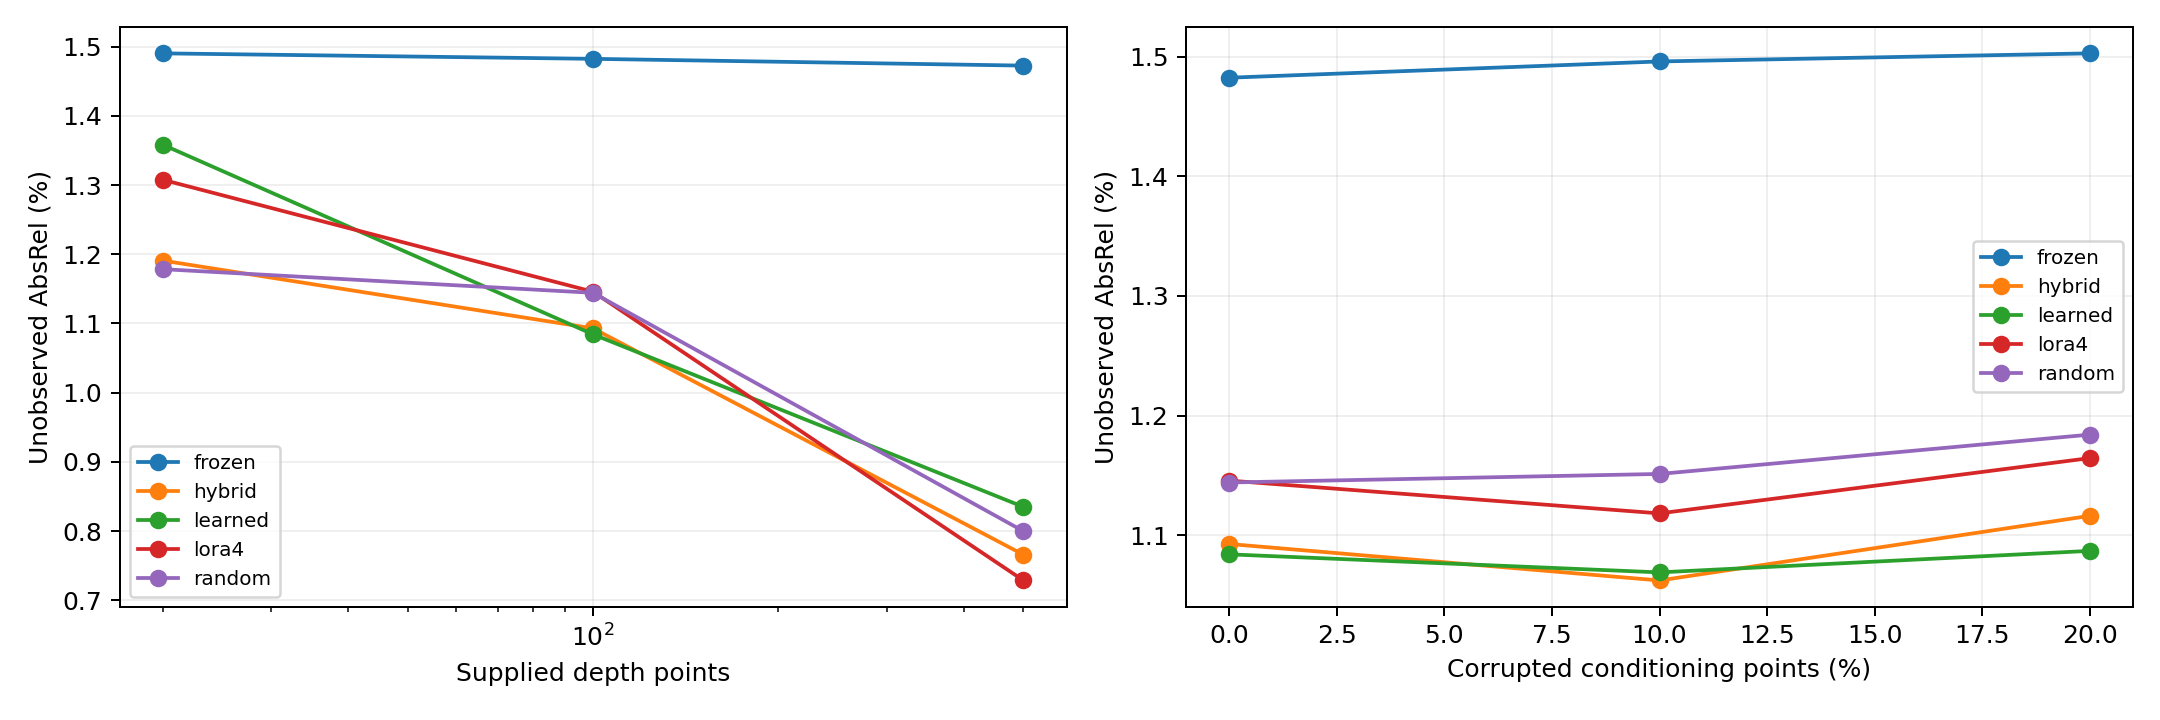
\includegraphics[width=\linewidth]{robustness.png}
  \caption{Unobserved AbsRel versus number of supplied depth points (left, log scale) and fraction of corrupted conditioning points (right). Learned bases are best at 100 points and stay flat under corruption, while LoRA overtakes them at 500 points.}
  \label{fig:robust}
\end{figure}

\begin{table}[h]
  \centering
  \small
  \begin{minipage}[t]{0.40\linewidth}
    \centering
    \caption{Attribute ablation on validation (unobs.\ AbsRel \%).}
    \label{tab:abl}
    \begin{tabular}{lc}
      \toprule
      Basis source & AbsRel $\downarrow$ \\
      \midrule
      \textbf{Geometry} & \textbf{1.0745} \\
      Texture & 1.2337 \\
      Camera & 1.2338 \\
      Combined & 1.2462 \\
      Lighting & 1.2675 \\
      \bottomrule
    \end{tabular}
  \end{minipage}\hfill
  \begin{minipage}[t]{0.56\linewidth}
    \centering
    \caption{Adaptation cost per test input.}
    \label{tab:eff}
    \begin{tabular}{lcc}
      \toprule
      Method & Time (s) & Peak mem.\ (GB) \\
      \midrule
      Rank-4 LoRA & 80.03 & 6.083 \\
      Robust bases & 79.53 & 6.080 \\
      Energy-pooled bases & 79.29 & 6.080 \\
      Bases + residual & 79.85 & 6.081 \\
      \bottomrule
    \end{tabular}
  \end{minipage}
\end{table}

\paragraph{Attribute ablation.} Table~\ref{tab:abl} compares individual attribute bases on validation data with equal basis dimensions and a common update budget. Geometry is \textbf{13.77\% better than the combined basis}, consistent with the geometric nature of depth completion, though not confirmed on an independent test set. Under a fixed four-dimensional capacity, merging attributes may dilute the most relevant directions, which motivates task-aware selection or adaptive basis dimensions.

\paragraph{Efficiency.} Table~\ref{tab:eff} shows that adaptation time and peak GPU memory are nearly identical across methods despite the large difference in trainable variables. Forward and backward passes through the foundation model dominate the cost, so the sub-1\% timing difference is not a reliable speedup. The demonstrated gain is \textbf{a much smaller trainable adaptation state with better mean accuracy}, not lower memory or latency. Timings exclude loading, preprocessing, metrics, saving, and offline donor training.

\section{Conclusion and limitations}

Reusing attribute-derived directions is supported within our small synthetic-to-real and real-donor study. Test-time trainable parameters drop from 393,216 to 384, and mean accuracy improves, most strongly with energy pooling. Sparse-observation benefits are condition-dependent: learned bases lead at 100 points but not at 20 or 500. Outlier robustness is encouraging under the tested corruption model. The residual LoRA helps in selected sparse conditions but adds little main-study accuracy. A constrained space reaches the optimum in the quadratic when the optimum lies inside it. Reduced real-model convergence time or runtime is \emph{not} established.

\textbf{Learning where to adapt is a promising route to parameter-efficient adaptation, provided the subspace and its flexibility match the task.} We do not claim universal superiority, semantic disentanglement, or global-optimum convergence in a foundation model. The study uses two donor, one validation, and two test sequences plus two procedural base scenes; repeated frames and seeds do not replace independent scenes, so results show feasibility rather than statistical significance. Pure fixed-basis coefficients start at zero for both seeds, so those repeats are not independent bases. Natural next steps are broader donor diversity, more held-out scenes, repeated corruption draws, task-aware attribute selection, adaptive basis dimensions, and time-to-accuracy comparisons that include the offline cost of building the bases.

\section*{References}
{
\small

[1] Depth Completion as Parameter-Efficient Test-Time Adaptation (CAPA). \url{https://arxiv.org/abs/2602.14751}. Code: \url{https://github.com/nv-dvl/capa}.

[2] Mining Attribute Subspaces for Efficient Fine-tuning of 3D Foundation Models. \url{https://arxiv.org/abs/2604.10095}.

[3] VGGT: Visual Geometry Grounded Transformer. \url{https://github.com/facebookresearch/vggt}.
}

\end{document}
